% Options for packages loaded elsewhere
% Options for packages loaded elsewhere
\PassOptionsToPackage{unicode}{hyperref}
\PassOptionsToPackage{hyphens}{url}
\PassOptionsToPackage{dvipsnames,svgnames,x11names}{xcolor}
%
\documentclass[
  russian,
  letterpaper,
  DIV=11,
  numbers=noendperiod]{scrartcl}
\usepackage{xcolor}
\usepackage{amsmath,amssymb}
\setcounter{secnumdepth}{5}
\usepackage{iftex}
\ifPDFTeX
  \usepackage[T1]{fontenc}
  \usepackage[utf8]{inputenc}
  \usepackage{textcomp} % provide euro and other symbols
\else % if luatex or xetex
  \usepackage{unicode-math} % this also loads fontspec
  \defaultfontfeatures{Scale=MatchLowercase}
  \defaultfontfeatures[\rmfamily]{Ligatures=TeX,Scale=1}
\fi
\usepackage{lmodern}
\ifPDFTeX\else
  % xetex/luatex font selection
\fi
% Use upquote if available, for straight quotes in verbatim environments
\IfFileExists{upquote.sty}{\usepackage{upquote}}{}
\IfFileExists{microtype.sty}{% use microtype if available
  \usepackage[]{microtype}
  \UseMicrotypeSet[protrusion]{basicmath} % disable protrusion for tt fonts
}{}
\makeatletter
\@ifundefined{KOMAClassName}{% if non-KOMA class
  \IfFileExists{parskip.sty}{%
    \usepackage{parskip}
  }{% else
    \setlength{\parindent}{0pt}
    \setlength{\parskip}{6pt plus 2pt minus 1pt}}
}{% if KOMA class
  \KOMAoptions{parskip=half}}
\makeatother
% Make \paragraph and \subparagraph free-standing
\makeatletter
\ifx\paragraph\undefined\else
  \let\oldparagraph\paragraph
  \renewcommand{\paragraph}{
    \@ifstar
      \xxxParagraphStar
      \xxxParagraphNoStar
  }
  \newcommand{\xxxParagraphStar}[1]{\oldparagraph*{#1}\mbox{}}
  \newcommand{\xxxParagraphNoStar}[1]{\oldparagraph{#1}\mbox{}}
\fi
\ifx\subparagraph\undefined\else
  \let\oldsubparagraph\subparagraph
  \renewcommand{\subparagraph}{
    \@ifstar
      \xxxSubParagraphStar
      \xxxSubParagraphNoStar
  }
  \newcommand{\xxxSubParagraphStar}[1]{\oldsubparagraph*{#1}\mbox{}}
  \newcommand{\xxxSubParagraphNoStar}[1]{\oldsubparagraph{#1}\mbox{}}
\fi
\makeatother


\usepackage{longtable,booktabs,array}
\usepackage{calc} % for calculating minipage widths
% Correct order of tables after \paragraph or \subparagraph
\usepackage{etoolbox}
\makeatletter
\patchcmd\longtable{\par}{\if@noskipsec\mbox{}\fi\par}{}{}
\makeatother
% Allow footnotes in longtable head/foot
\IfFileExists{footnotehyper.sty}{\usepackage{footnotehyper}}{\usepackage{footnote}}
\makesavenoteenv{longtable}
\usepackage{graphicx}
\makeatletter
\newsavebox\pandoc@box
\newcommand*\pandocbounded[1]{% scales image to fit in text height/width
  \sbox\pandoc@box{#1}%
  \Gscale@div\@tempa{\textheight}{\dimexpr\ht\pandoc@box+\dp\pandoc@box\relax}%
  \Gscale@div\@tempb{\linewidth}{\wd\pandoc@box}%
  \ifdim\@tempb\p@<\@tempa\p@\let\@tempa\@tempb\fi% select the smaller of both
  \ifdim\@tempa\p@<\p@\scalebox{\@tempa}{\usebox\pandoc@box}%
  \else\usebox{\pandoc@box}%
  \fi%
}
% Set default figure placement to htbp
\def\fps@figure{htbp}
\makeatother



\ifLuaTeX
\usepackage[bidi=basic,provide=*]{babel}
\else
\usepackage[bidi=default,provide=*]{babel}
\fi
% get rid of language-specific shorthands (see #6817):
\let\LanguageShortHands\languageshorthands
\def\languageshorthands#1{}


\setlength{\emergencystretch}{3em} % prevent overfull lines

\providecommand{\tightlist}{%
  \setlength{\itemsep}{0pt}\setlength{\parskip}{0pt}}



 


\usepackage{fontspec}

\setsansfont{Palatino Linotype}[
    Path=../files/palatino/,
    Extension = .ttf,
    UprightFont=palatino-Roman,
    BoldFont=palatino-Bold,
    ItalicFont=palatino-Italic,
    BoldItalicFont=palatino-BoldItalic
]
\setmainfont{Palatino Linotype}[
    Path=../files/palatino/,
    Extension = .ttf,
    UprightFont=palatino-Roman,
    BoldFont=palatino-Bold,
    ItalicFont=palatino-Italic,
    BoldItalicFont=palatino-BoldItalic
]

\usepackage[textwidth=0.86\paperwidth, textheight=0.86\paperheight]{geometry}
\usepackage{fancyhdr}
\usepackage{hyperref}
\usepackage{fontawesome5}
\usepackage{graphicx}
\usepackage{amssymb}
\usepackage{amsmath}
\graphicspath{{../files/}}

\newcommand{\R}{\mathbb{R}}

% \pagenumbering{gobble}
\pagestyle{fancy}
\fancyhead{} % clear all header fields
\fancyhead[R]{\href{https://cu25.fmin.xyz}{\faGem[regular]} \hspace{0.04cm} \href{https://github.com/MerkulovDaniil/cu25}{\faGithub} \hspace{0.07cm} \href{https://t.me/fminxyz}{\faTelegram}}
\fancyhead[L]{\href{https://fmin.xyz}{
\includegraphics[height=0.35cm]{logo.pdf}} ~ 
\includegraphics[height=0.35cm]{logo_cu.pdf} \hspace{2pt} \textbf{Оптимизация для всех! ЦУ. 2025}}
\KOMAoption{captions}{tableheading}
\makeatletter
\@ifpackageloaded{tcolorbox}{}{\usepackage[skins,breakable]{tcolorbox}}
\@ifpackageloaded{fontawesome5}{}{\usepackage{fontawesome5}}
\definecolor{quarto-callout-color}{HTML}{909090}
\definecolor{quarto-callout-note-color}{HTML}{0758E5}
\definecolor{quarto-callout-important-color}{HTML}{CC1914}
\definecolor{quarto-callout-warning-color}{HTML}{EB9113}
\definecolor{quarto-callout-tip-color}{HTML}{00A047}
\definecolor{quarto-callout-caution-color}{HTML}{FC5300}
\definecolor{quarto-callout-color-frame}{HTML}{acacac}
\definecolor{quarto-callout-note-color-frame}{HTML}{4582ec}
\definecolor{quarto-callout-important-color-frame}{HTML}{d9534f}
\definecolor{quarto-callout-warning-color-frame}{HTML}{f0ad4e}
\definecolor{quarto-callout-tip-color-frame}{HTML}{02b875}
\definecolor{quarto-callout-caution-color-frame}{HTML}{fd7e14}
\makeatother
\makeatletter
\@ifpackageloaded{caption}{}{\usepackage{caption}}
\AtBeginDocument{%
\ifdefined\contentsname
  \renewcommand*\contentsname{Содержание}
\else
  \newcommand\contentsname{Содержание}
\fi
\ifdefined\listfigurename
  \renewcommand*\listfigurename{Список Иллюстраций}
\else
  \newcommand\listfigurename{Список Иллюстраций}
\fi
\ifdefined\listtablename
  \renewcommand*\listtablename{Список Таблиц}
\else
  \newcommand\listtablename{Список Таблиц}
\fi
\ifdefined\figurename
  \renewcommand*\figurename{Рисунок}
\else
  \newcommand\figurename{Рисунок}
\fi
\ifdefined\tablename
  \renewcommand*\tablename{Таблица}
\else
  \newcommand\tablename{Таблица}
\fi
}
\@ifpackageloaded{float}{}{\usepackage{float}}
\floatstyle{ruled}
\@ifundefined{c@chapter}{\newfloat{codelisting}{h}{lop}}{\newfloat{codelisting}{h}{lop}[chapter]}
\floatname{codelisting}{Список}
\newcommand*\listoflistings{\listof{codelisting}{Список Каталогов}}
\makeatother
\makeatletter
\makeatother
\makeatletter
\@ifpackageloaded{caption}{}{\usepackage{caption}}
\@ifpackageloaded{subcaption}{}{\usepackage{subcaption}}
\makeatother
\usepackage{bookmark}
\IfFileExists{xurl.sty}{\usepackage{xurl}}{} % add URL line breaks if available
\urlstyle{same}
\hypersetup{
  pdftitle={Градиентный спуск. Теоремы сходимости в гладком случае (выпуклые, сильно выпуклые, PL). Верхние и нижние оценки сходимости.},
  pdfauthor={Даня Меркулов},
  pdflang={ru},
  colorlinks=true,
  linkcolor={blue},
  filecolor={Maroon},
  citecolor={Blue},
  urlcolor={Blue},
  pdfcreator={LaTeX via pandoc}}


\title{Градиентный спуск. Теоремы сходимости в гладком случае (выпуклые,
сильно выпуклые, PL). Верхние и нижние оценки сходимости.}
\author{Даня Меркулов}
\date{}
\begin{document}
\maketitle


\section{Градиентный
спуск}\label{ux433ux440ux430ux434ux438ux435ux43dux442ux43dux44bux439-ux441ux43fux443ux441ux43a}

\subsection{Направление локального наискорейшего
спуска}\label{ux43dux430ux43fux440ux430ux432ux43bux435ux43dux438ux435-ux43bux43eux43aux430ux43bux44cux43dux43eux433ux43e-ux43dux430ux438ux441ux43aux43eux440ux435ux439ux448ux435ux433ux43e-ux441ux43fux443ux441ux43aux430}

Рассмотрим линейное приближение дифференцируемой функции \(f\) вдоль
направления \(h\), где \(\|h\|_2 = 1\):

\[
f(x + \alpha h) = f(x) + \alpha \langle \nabla f(x), h \rangle + o(\alpha)
\]

Хотим, чтобы \(h\) было направлением убывания: \[
f(x + \alpha h) < f(x)
\] \[
f(x) + \alpha \langle \nabla f(x), h \rangle + o(\alpha) < f(x)
\]

Переходя к пределу при \(\alpha \to 0\): \[
\langle \nabla f(x), h \rangle \leq 0
\]

Также из неравенства Коши--Буняковского получаем: \[
\begin{split}
|\langle \nabla f(x), h \rangle | &\leq \| \nabla f(x) \|_2 \| h \|_2 \\
\langle \nabla f(x), h \rangle &\geq -\| \nabla f(x) \|_2 \| h \|_2 = -\| \nabla f(x) \|_2
\end{split}
\]

Таким образом, направление антиградиента \[
h = -\dfrac{\nabla f(x)}{\|\nabla f(x)\|_2}
\] представляет собой направление \textbf{наискорейшего локального}
убывания функции \(f\).

Итерация метода имеет вид: \[
x^{k+1} = x^k - \alpha \, \nabla f(x^k)
\]

\subsection{Дифференциальное уравнение градиентного
потока}\label{ux434ux438ux444ux444ux435ux440ux435ux43dux446ux438ux430ux43bux44cux43dux43eux435-ux443ux440ux430ux432ux43dux435ux43dux438ux435-ux433ux440ux430ux434ux438ux435ux43dux442ux43dux43eux433ux43e-ux43fux43eux442ux43eux43aux430}

Рассмотрим дифференциальное уравнение градиентного потока: \[
\tag{GF}
\frac{dx}{dt} = -\nabla f(x(t)).
\]

Дискретизируем его на равномерной сетке с шагом \(\alpha\): \[
\frac{x^{k+1} - x^k}{\alpha} = -\nabla f(x^k),
\]

где \(x^k \equiv x(t_k)\) и \(\alpha = t_{k+1} - t_k\) --- шаг сетки.

Отсюда получаем выражение для \(x^{k+1}\): \[
x^{k+1} = x^k - \alpha \, \nabla f(x^k),
\] являющееся точной формулой обновления градиентного спуска.

\href{https://colab.research.google.com/github/MerkulovDaniil/optim/blob/master/assets/Notebooks/GD_vs_GF.ipynb}{Открыть
в Colab \(\clubsuit\)}

\begin{figure}[H]

{\centering \pandocbounded{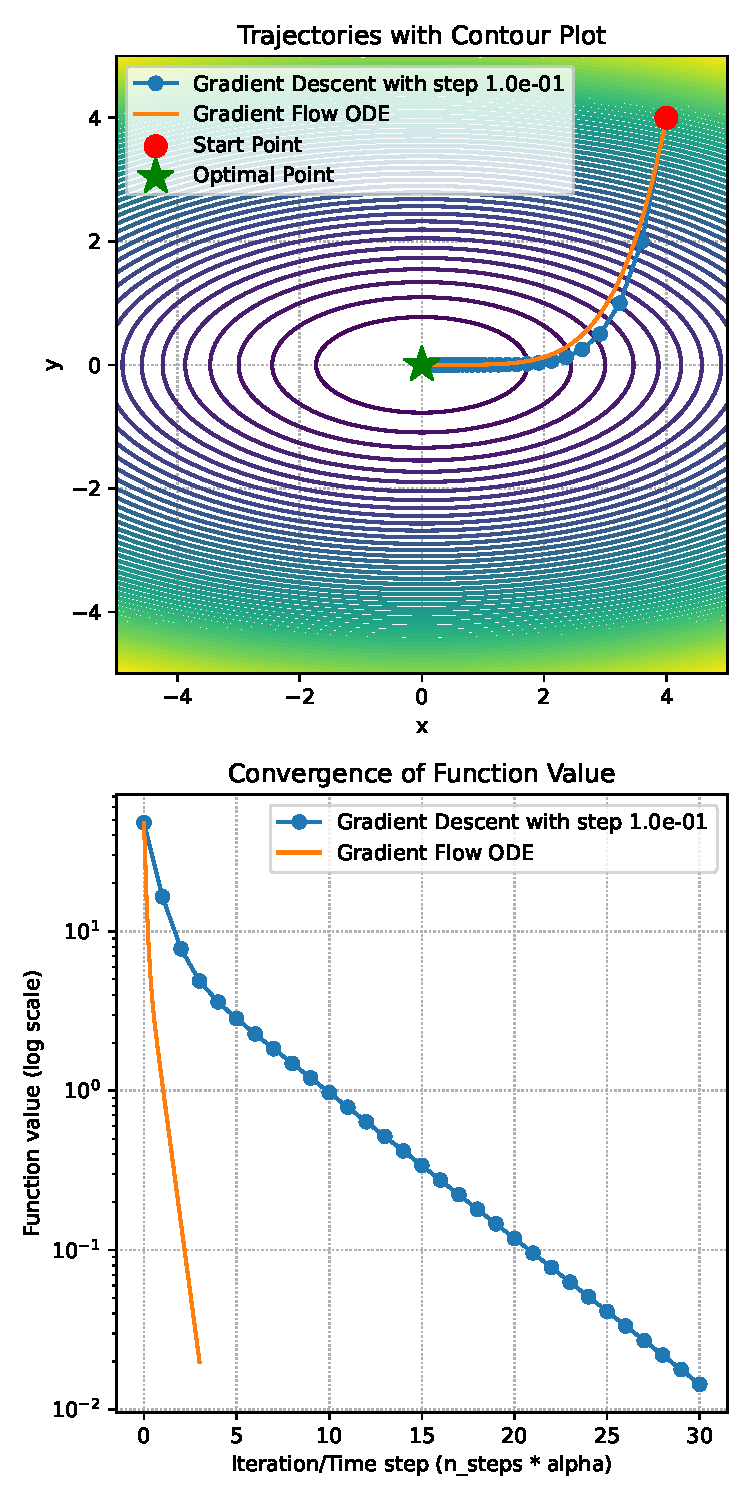
\includegraphics[keepaspectratio]{GD_vs_GF.pdf}}

}

\caption{Траектория градиентного потока}

\end{figure}%

\subsection{Сходимость алгоритма градиентного
спуска}\label{ux441ux445ux43eux434ux438ux43cux43eux441ux442ux44c-ux430ux43bux433ux43eux440ux438ux442ux43cux430-ux433ux440ux430ux434ux438ux435ux43dux442ux43dux43eux433ux43e-ux441ux43fux443ux441ux43aux430}

\href{https://colab.research.google.com/github/MerkulovDaniil/optim/blob/master/assets/Notebooks/GD_2d_visualization.ipynb}{\faPython Код}
для построения анимации ниже. Сходимость существенно зависит от выбора
шага \(\alpha\):

\href{https://fmin.xyz/docs/visualizations/gd_lls.mp4}{\pandocbounded{
\includegraphics[keepaspectratio]{gd_2d.png}}}

\subsection{Точный линейный поиск (метод наискорейшего
спуска)}\label{ux442ux43eux447ux43dux44bux439-ux43bux438ux43dux435ux439ux43dux44bux439-ux43fux43eux438ux441ux43a-ux43cux435ux442ux43eux434-ux43dux430ux438ux441ux43aux43eux440ux435ux439ux448ux435ux433ux43e-ux441ux43fux443ux441ux43aux430}

\[
\alpha_k = \operatorname*{arg\,min}_{\alpha \in \mathbb{R}^+} f\bigl(x^k - \alpha \, \nabla f(x^k)\bigr)
\] Подход скорее теоретический, чем практический: он удобен для анализа
сходимости, но точный линейный поиск часто затруднён, если вычисление
функции занимает слишком много времени или стоит слишком дорого.

Интересное теоретическое свойство этого метода заключается в том, что
градиенты на соседних итерациях ортогональны. Условие оптимальности по
\(\alpha_k\) даёт \[
\left.\dfrac{d}{d\alpha} \, f\bigl(x^k - \alpha \, \nabla f(x^k)\bigr)\right|_{\alpha = \alpha_k} = 0.
\]

Условия оптимальности:

\[
\nabla f(x^{k+1})^\top \nabla f(x^k) = 0
\]

\begin{figure}[H]

{\centering \pandocbounded{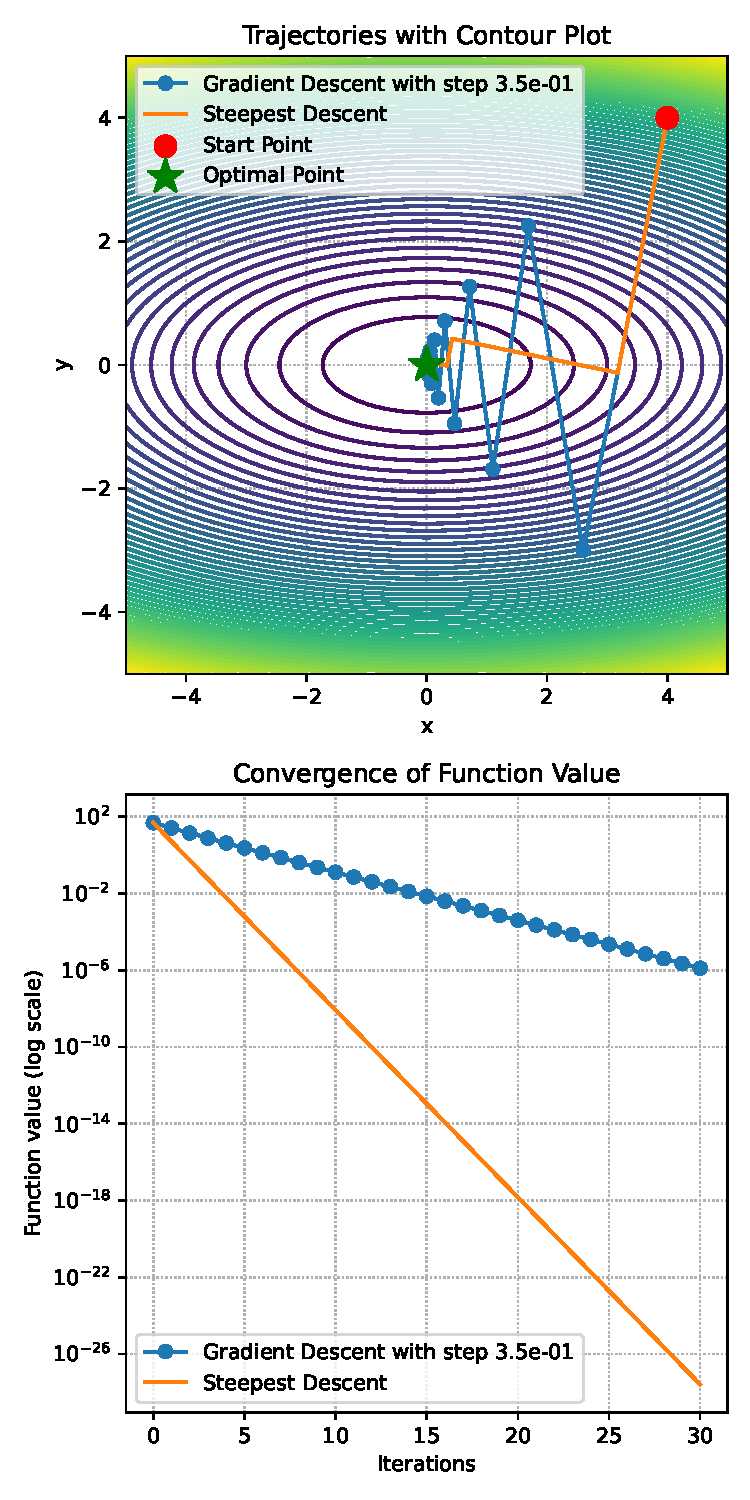
\includegraphics[keepaspectratio]{GD_vs_Steepest.pdf}}

}

\caption{Наискорейший спуск}

\end{figure}%

\href{https://colab.research.google.com/github/MerkulovDaniil/optim/blob/master/assets/Notebooks/Steepest_descent.ipynb}{Открыть
в Colab \(\clubsuit\)}

\section{Сильно выпуклые квадратичные
функции}\label{ux441ux438ux43bux44cux43dux43e-ux432ux44bux43fux443ux43aux43bux44bux435-ux43aux432ux430ux434ux440ux430ux442ux438ux447ux43dux44bux435-ux444ux443ux43dux43aux446ux438ux438}

\subsection{Сдвиг
координат}\label{ux441ux434ux432ux438ux433-ux43aux43eux43eux440ux434ux438ux43dux430ux442}

Рассмотрим следующую задачу квадратичной оптимизации: \[
\label{problem}
\min\limits_{x \in \mathbb{R}^d} f(x) =  \min\limits_{x \in \mathbb{R}^d} \dfrac{1}{2} x^\top  A x - b^\top  x + c, \text{ где } A \in \mathbb{S}^d_{++}.
\]

\begin{itemize}
\tightlist
\item
  Во-первых, без ограничения общности мы можем установить \(c = 0\), что
  не повлияет на процесс оптимизации.
\item
  Во-вторых, у нас есть спектральное разложение матрицы
  \(A = Q \Lambda Q^T\).
\item
  Покажем, что мы можем сделать сдвиг координат, чтобы сделать анализ
  немного проще. Пусть \(\hat{x} = Q^T(x - x^*)\), где \(x^*\) --- точка
  минимума исходной функции, определяемая как \(Ax^* = b\). При этом
  \(x = Q\hat{x} + x^*\). \[
    \begin{split}
     f(\hat{x}) &= \frac12  (Q\hat{x} + x^*)^\top  A (Q\hat{x} + x^*) - b^\top  (Q\hat{x} + x^*) \\
     &= \frac12 \hat{x}^T Q^TAQ\hat{x} + \frac12 (x^*)^T A (x^*) + (x^*)^TAQ\hat{x} - b^T Q\hat{x} - b^T x^*\\
     &= \frac12 \hat{x}^T \Lambda \hat{x} + \frac12 (x^*)^T A (x^*) + (x^*)^TAQ\hat{x} - (x^*)^T A^TQ\hat{x} - (x^*)^T A x^*\\
    &= \frac12 \hat{x}^T \Lambda \hat{x} - \frac12 (x^*)^T A x^* \simeq \frac12 \hat{x}^T \Lambda \hat{x} 
    \end{split}
    \]
\end{itemize}

\pandocbounded{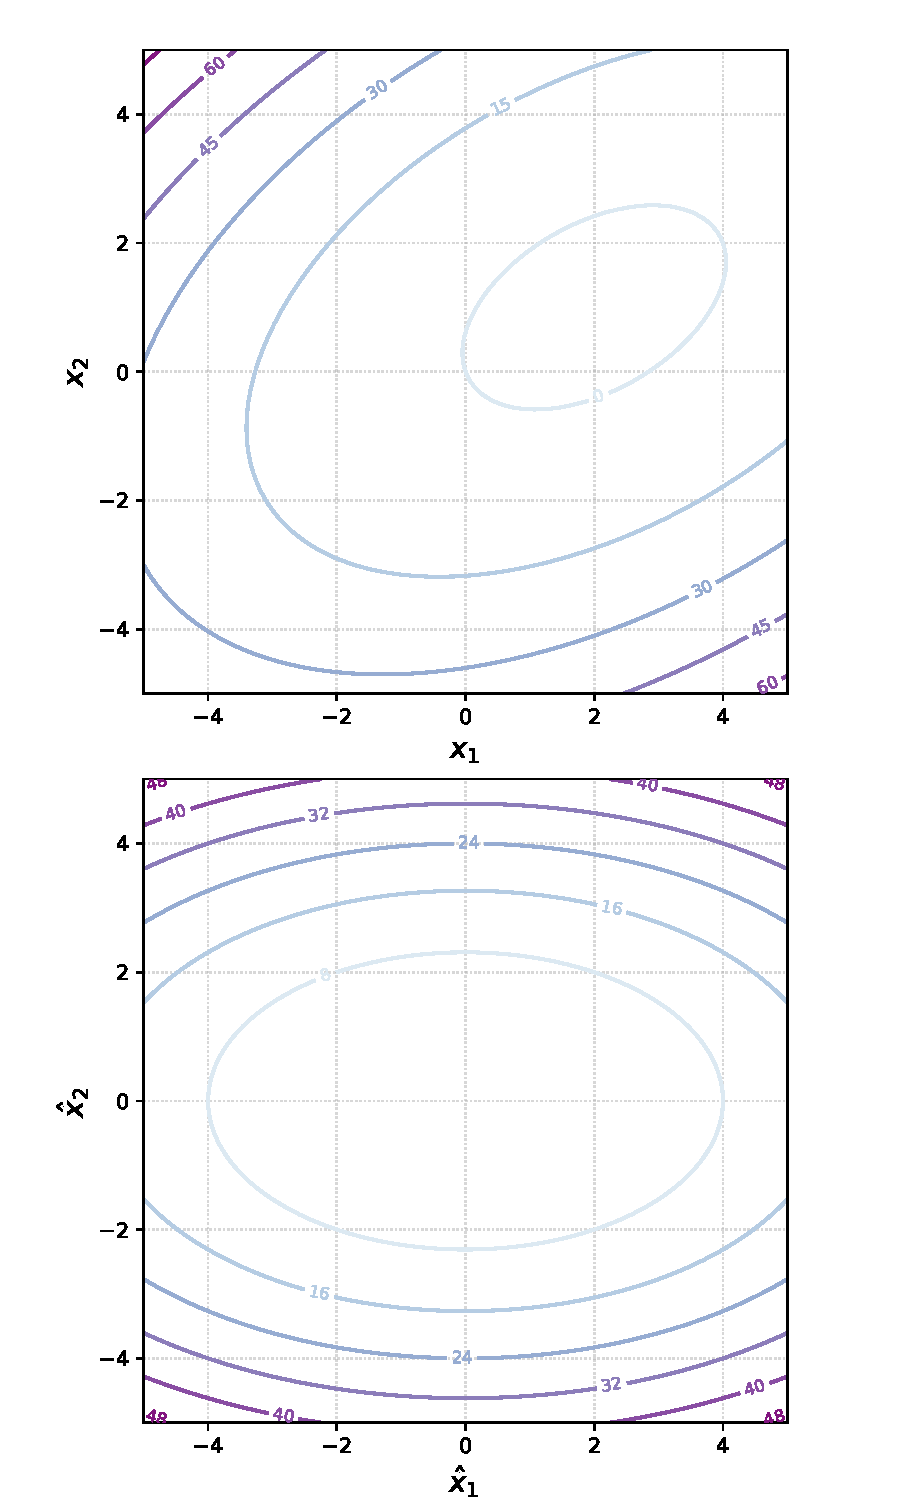
\includegraphics[keepaspectratio]{coordinate_shift.pdf}}

\subsection{Анализ
сходимости}\label{ux430ux43dux430ux43bux438ux437-ux441ux445ux43eux434ux438ux43cux43eux441ux442ux438}

Теперь мы можем работать с функцией \(f(x) = \frac12 x^T \Lambda x\) с
\(x^* = 0\) без ограничения общности (убрав крышку из \(\hat{x}\))

\[
\begin{split}
x^{k+1} &= x^k - \alpha^k \nabla f(x^k)
= x^k - \alpha^k \Lambda x^k \\  
&= (I - \alpha^k \Lambda) x^k \\ 
x^{k+1}_{(i)} &= (1 - \alpha^k \lambda_{(i)}) \, x^k_{(i)} \quad \text{для $i$-й координаты} \\ 
x^{k}_{(i)} &= (1 - \alpha \, \lambda_{(i)})^k \, x^0_{(i)} \quad \text{при постоянном шаге } \alpha^k = \alpha
\end{split}
\]

Используем постоянный шаг \(\alpha^k = \alpha\). Условие сходимости: \[
\rho(\alpha) = \max_{i} |1 - \alpha \lambda_{(i)}| < 1
\]

Помним, что \(\lambda_{\min} = \mu > 0\),
\(\lambda_{\max} = L \geq \mu\).

\[
\begin{split}
|1 - \alpha \mu| &< 1 \\ 
 -1 < 1 &- \alpha \mu < 1 \\ 
 \alpha < \tfrac{2}{\mu} \quad & \quad \alpha\mu > 0
\end{split}
\]

\[
\begin{split}
|1 - \alpha L| &< 1 \\ 
 -1 < 1 &- \alpha L < 1 \\ 
 \alpha < \tfrac{2}{L} \quad & \quad \alpha L > 0
\end{split}
\]

Выберем \(\alpha\), минимизирующий худший знаменатель прогрессии \[
\begin{split}
\rho^* &=  \min_{\alpha} \rho(\alpha)   = \min_{\alpha} \max_{i} |1 - \alpha \lambda_{(i)}| \\ 
 &=  \min_{\alpha} \left\{|1 - \alpha \mu|, |1 - \alpha L| \right\} \\ 
\alpha^* &: \quad  1 - \alpha^* \mu = \alpha^* L - 1 \\ 
 & \alpha^* = \frac{2}{\mu + L}  \quad \rho^* = \frac{L - \mu}{L + \mu} \\ 
 |x^{k}_{(i)}| &\leq \left( \frac{L - \mu}{L + \mu} \right)^k |x^0_{(i)}| \\
 \|x^{k}\|_2 &\leq \left( \frac{L - \mu}{L + \mu} \right)^k \|x^0\|_2  \quad f(x^{k}) \leq \left( \frac{L - \mu}{L + \mu} \right)^{2k} f(x^0)
\end{split}
\]

Таким образом, имеем линейную сходимость по аргументу со скоростью
\(\frac{\varkappa - 1}{\varkappa + 1} = 1 - \frac{2}{\varkappa + 1}\),
где \(\varkappa = \frac{L}{\mu}\) --- \emph{число обусловленности}
квадратичной задачи.

\begin{longtable}[]{@{}
  >{\centering\arraybackslash}p{(\linewidth - 6\tabcolsep) * \real{0.0938}}
  >{\centering\arraybackslash}p{(\linewidth - 6\tabcolsep) * \real{0.0938}}
  >{\centering\arraybackslash}p{(\linewidth - 6\tabcolsep) * \real{0.4062}}
  >{\centering\arraybackslash}p{(\linewidth - 6\tabcolsep) * \real{0.4062}}@{}}
\toprule\noalign{}
\begin{minipage}[b]{\linewidth}\centering
\(\varkappa\)
\end{minipage} & \begin{minipage}[b]{\linewidth}\centering
\(\rho\)
\end{minipage} & \begin{minipage}[b]{\linewidth}\centering
Итераций до уменьшения ошибки по аргументу в \(10\) раз
\end{minipage} & \begin{minipage}[b]{\linewidth}\centering
Итераций до уменьшения ошибки по функции в \(10\) раз
\end{minipage} \\
\midrule\noalign{}
\endhead
\bottomrule\noalign{}
\endlastfoot
\(1.1\) & \(0.05\) & \(1\) & \(1\) \\
\(2\) & \(0.33\) & \(3\) & \(2\) \\
\(5\) & \(0.67\) & \(6\) & \(3\) \\
\(10\) & \(0.82\) & \(12\) & \(6\) \\
\(50\) & \(0.96\) & \(58\) & \(29\) \\
\(100\) & \(0.98\) & \(116\) & \(58\) \\
\(500\) & \(0.996\) & \(576\) & \(288\) \\
\(1000\) & \(0.998\) & \(1152\) & \(576\) \\
\end{longtable}

\subsection{\texorpdfstring{Число обусловленности
\(\varkappa\)}{Число обусловленности \textbackslash varkappa}}\label{ux447ux438ux441ux43bux43e-ux43eux431ux443ux441ux43bux43eux432ux43bux435ux43dux43dux43eux441ux442ux438-varkappa}

\href{https://fmin.xyz/docs/visualizations/condition_number_gd.mp4}{\pandocbounded{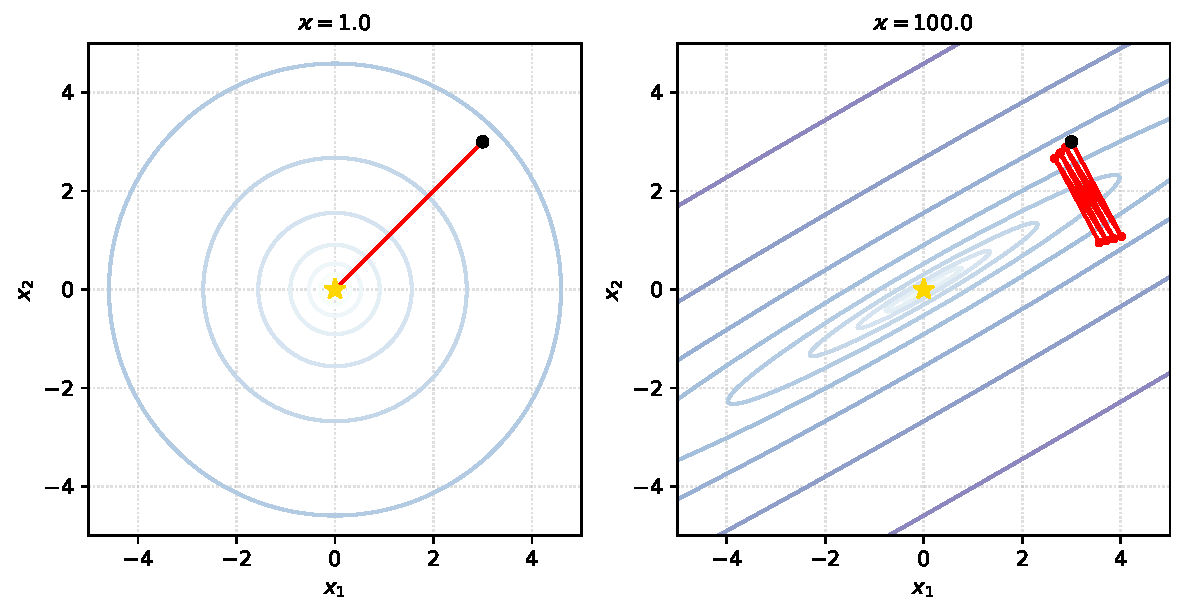
\includegraphics[keepaspectratio]{condition_number_gd.pdf}}}

\section{Случай
PL-функций}\label{ux441ux43bux443ux447ux430ux439-pl-ux444ux443ux43dux43aux446ux438ux439}

\subsection{PL-функции. Линейная сходимость градиентного спуска без
выпуклости}\label{pl-ux444ux443ux43dux43aux446ux438ux438.-ux43bux438ux43dux435ux439ux43dux430ux44f-ux441ux445ux43eux434ux438ux43cux43eux441ux442ux44c-ux433ux440ux430ux434ux438ux435ux43dux442ux43dux43eux433ux43e-ux441ux43fux443ux441ux43aux430-ux431ux435ux437-ux432ux44bux43fux443ux43aux43bux43eux441ux442ux438}

Говорят, что \(f\) удовлетворяет условию Поляка-Лоясиевича (PL), если
для некоторого \(\mu > 0\) выполняется \[
\Vert \nabla f(x) \Vert^2 \geq 2 \mu (f(x) - f^*) \quad \forall x
\] Интересно, что градиентный спуск может сходиться линейно даже без
выпуклости.

Следующие функции удовлетворяют условию PL, но не являются выпуклыми.
\href{https://colab.research.google.com/github/MerkulovDaniil/optim/blob/master/assets/Notebooks/PL_function.ipynb}{\faPython Код}

\[
f(x) = x^2 + 3\sin^2(x)
\]

\begin{figure}[H]

{\centering 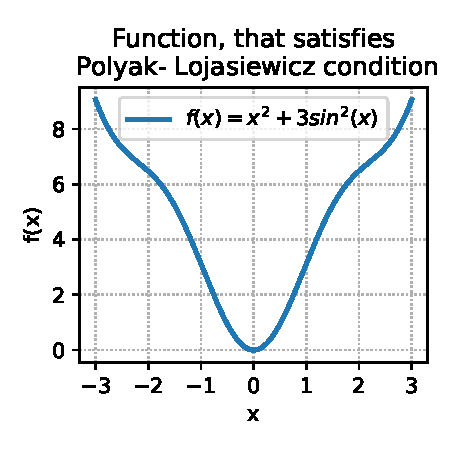
\includegraphics[width=0.5\linewidth,height=\textheight,keepaspectratio]{pl_2d.pdf}

}

\caption{PL-функция}

\end{figure}%

\[
f(x,y) = \dfrac{(y - \sin x)^2}{2}
\]

\begin{figure}[H]

{\centering 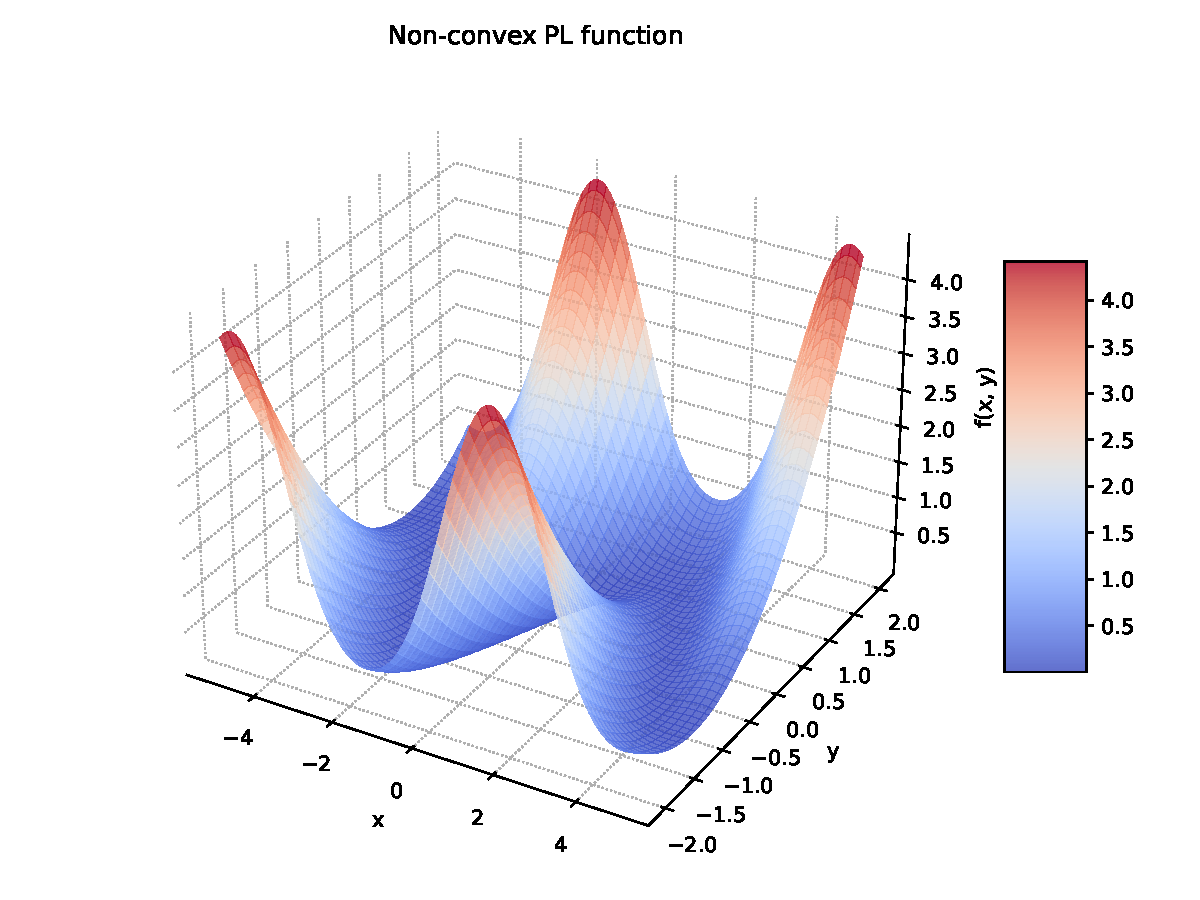
\includegraphics[width=0.5\linewidth,height=\textheight,keepaspectratio]{pl_3d.pdf}

}

\caption{PL-функция}

\end{figure}%

\subsection{Анализ
сходимости}\label{ux430ux43dux430ux43bux438ux437-ux441ux445ux43eux434ux438ux43cux43eux441ux442ux438-1}

\begin{tcolorbox}[enhanced jigsaw, bottomrule=.15mm, coltitle=black, opacitybacktitle=0.6, colbacktitle=quarto-callout-color!10!white, colback=white, opacityback=0, toprule=.15mm, bottomtitle=1mm, toptitle=1mm, arc=.35mm, title=\textcolor{quarto-callout-color}{\faInfo}\hspace{0.5em}{Theorem}, titlerule=0mm, rightrule=.15mm, leftrule=.75mm, left=2mm, colframe=quarto-callout-color-frame, breakable]

Рассмотрим задачу \[
f(x) \to \min_{x \in \mathbb{R}^d}
\] и предположим, что \(f\) является PL-функцией с константой \(\mu\) и
\(L\)-гладкой, для некоторых \(L\geq \mu > 0\).

Рассмотрим последовательность \((x^k)_{k \in \mathbb{N}}\),
сгенерированную методом градиентного спуска из точки \(x^0\) с
постоянным шагом \(\alpha\), удовлетворяющим
\(0<\alpha \leq \frac{1}{L}\). Пусть
\(f^* = \min\limits_{x \in \mathbb{R}^d} f(x)\). Тогда: \[
f(x^{k})-f^* \leq (1-\alpha \mu)^k (f(x^0)-f^*).
\]

\end{tcolorbox}

Используем \(L\)-гладкость вместе с правилом обновления, чтобы записать:
\[
\begin{split}
 f(x^{k+1})& \leq f(x^{k}) + \langle \nabla f(x^{k}), x^{k+1}-x^{k} \rangle +\frac{L}{2} \| x^{k+1}-x^{k}\|^2\\ 
 &= f(x^{k})-\alpha\Vert \nabla f(x^{k}) \Vert^2 +\frac{L \alpha^2}{2} \| \nabla f(x^{k})\|^2 \\ 
 &= f(x^{k}) - \frac{\alpha}{2} \left(2 - L \alpha \right)\Vert \nabla f(x^{k}) \Vert^2 \\ 
 & \leq f(x^{k}) - \frac{\alpha}{2}\Vert \nabla f(x^{k})\Vert^2,
\end{split}
\]

где в последнем неравенстве использована гипотеза о шаге
\(\alpha L \leq 1\).

Теперь используем свойство PL-функции и получаем: \[
f(x^{k+1}) \leq f(x^{k}) - \alpha \mu (f(x^{k}) - f^*).
\] Вычтя \(f^*\) из обеих частей этого неравенства и применив рекурсию,
мы получим искомый результат.

\subsection{\texorpdfstring{Любая \(\mu\)-сильно выпуклая
дифференцируемая функция является
PL-функцией}{Любая \textbackslash mu-сильно выпуклая дифференцируемая функция является PL-функцией}}\label{ux43bux44eux431ux430ux44f-mu-ux441ux438ux43bux44cux43dux43e-ux432ux44bux43fux443ux43aux43bux430ux44f-ux434ux438ux444ux444ux435ux440ux435ux43dux446ux438ux440ux443ux435ux43cux430ux44f-ux444ux443ux43dux43aux446ux438ux44f-ux44fux432ux43bux44fux435ux442ux441ux44f-pl-ux444ux443ux43dux43aux446ux438ux435ux439}

\begin{tcolorbox}[enhanced jigsaw, bottomrule=.15mm, coltitle=black, opacitybacktitle=0.6, colbacktitle=quarto-callout-color!10!white, colback=white, opacityback=0, toprule=.15mm, bottomtitle=1mm, toptitle=1mm, arc=.35mm, title=\textcolor{quarto-callout-color}{\faInfo}\hspace{0.5em}{Theorem}, titlerule=0mm, rightrule=.15mm, leftrule=.75mm, left=2mm, colframe=quarto-callout-color-frame, breakable]

Если функция \(f(x)\) дифференцируема и \(\mu\)-сильно выпукла, то она
является PL-функцией.

\end{tcolorbox}

\textbf{Доказательство}

По критерию сильной выпуклости первого порядка: \[
f(y) \geq f(x) + \nabla f(x)^T(y-x) + \tfrac{\mu}{2}\|y-x\|_2^2
\] Положим \(y = x^*\): \[
\begin{split}
 f(x^*) &\geq f(x) + \nabla f(x)^T(x^*-x) + \tfrac{\mu}{2}\|x^*-x\|_2^2 \\ 
f(x) - f(x^*) &\leq \nabla f(x)^T(x-x^*) - \tfrac{\mu}{2}\|x^*-x\|_2^2 = \\ 
&= \left(\nabla f(x)^T - \tfrac{\mu}{2}(x^*-x)\right)^T (x-x^*) = \\ 
&= \frac12 \left(\tfrac{2}{\sqrt{\mu}}\nabla f(x)^T - \sqrt{\mu}(x^*-x)\right)^T \sqrt{\mu}(x-x^*)\\ 
\end{split}
\]

Пусть \(a = \frac{1}{\sqrt{\mu}}\nabla f(x)\) и
\(b =\sqrt{\mu}(x-x^*) -\frac{1}{\sqrt{\mu}}\nabla f(x)\)

Тогда \(a+b = \sqrt{\mu}(x-x^*)\) и
\(a-b=\frac{2}{\sqrt{\mu}}\nabla f(x)-\sqrt{\mu}(x-x^*)\)

\[
\begin{split}
f(x) - f(x^*) &\leq \frac12 \left(\frac{1}{\mu}\|\nabla f(x)\|^2_2 - \left\|\sqrt{\mu}(x-x^*) -\frac{1}{\sqrt{\mu}}\nabla f(x)\right\|_2^2\right) \\ 
    f(x) - f(x^*) &\leq \frac{1}{2\mu}\|\nabla f(x)\|^2_2, \\ 
    \end{split}
    \]

которое является точным условием PL. Это означает, что мы уже имеем
доказательство линейной сходимости для любой сильно выпуклой функции.

\section{Выпуклый гладкий
случай}\label{ux432ux44bux43fux443ux43aux43bux44bux439-ux433ux43bux430ux434ux43aux438ux439-ux441ux43bux443ux447ux430ux439}

\begin{tcolorbox}[enhanced jigsaw, bottomrule=.15mm, coltitle=black, opacitybacktitle=0.6, colbacktitle=quarto-callout-color!10!white, colback=white, opacityback=0, toprule=.15mm, bottomtitle=1mm, toptitle=1mm, arc=.35mm, title=\textcolor{quarto-callout-color}{\faInfo}\hspace{0.5em}{Theorem}, titlerule=0mm, rightrule=.15mm, leftrule=.75mm, left=2mm, colframe=quarto-callout-color-frame, breakable]

Рассмотрим задачу \[
f(x) \to \min_{x \in \mathbb{R}^d}
\] и предположим, что \(f\) является выпуклой и \(L\)-гладкой функцией,
для некоторого \(L>0\).

Пусть \((x^{k})_{k \in \mathbb{N}}\) --- последовательность итераций,
сгенерированная методом градиентного спуска из точки \(x^0\) с
постоянным шагом \(\alpha\), удовлетворяющим
\(0 < \alpha\leq \frac{1}{L}\). Пусть
\(f^* = \min\limits_{x \in \mathbb{R}^d} f(x)\). Тогда для всех
\(x^* \in \operatorname*{arg\,min}\, f\) и всех \(k \in \mathbb{N}\)
справедливо: \[
f(x^{k})-f^* \leq \frac{\|x^0-x^*\| ^2}{2 \alpha k}.
\]

\end{tcolorbox}

\subsection{Анализ
сходимости}\label{ux430ux43dux430ux43bux438ux437-ux441ux445ux43eux434ux438ux43cux43eux441ux442ux438-2}

\begin{itemize}
\item
  Как и раньше, сначала используем гладкость:
  \begin{equation}\phantomsection\label{eq-gd-cs-smoothness}{
    \begin{split}
     f(x^{k+1})& \leq f(x^{k}) + \langle \nabla f(x^{k}), x^{k+1}-x^{k} \rangle +\frac{L}{2} \| x^{k+1}-x^{k}\|^2\\ 
     &= f(x^{k})-\alpha\Vert \nabla f(x^{k}) \Vert^2 +\frac{L \alpha^2}{2} \| \nabla f(x^{k})\|^2 \\ 
     &= f(x^{k}) - \frac{\alpha}{2} \left(2 - L \alpha \right)\Vert \nabla f(x^{k}) \Vert^2 \\ 
     & \leq f(x^{k}) - \frac{\alpha}{2}\Vert \nabla f(x^{k})\Vert^2, \\ 
     f(x^{k}) - f(x^{k+1}) & \geq \dfrac{1}{2L} \Vert \nabla f(x^{k})\Vert^2 \quad \text{если } \alpha = \tfrac1L 
    \end{split}
    }\end{equation}

  Обычно для сходящегося градиентного спуска чем больше допустимый шаг,
  тем быстрее сходимость, поэтому часто берут \(\alpha = \tfrac1L\).
\item
  После этого используем выпуклость:
  \begin{equation}\phantomsection\label{eq-gd-cs-convexity}{
   \begin{split}
   f(y) &\geq f(x) + \langle \nabla f(x), y-x\rangle \text{ где } y = x^*, x = x^k\\
   f(x^k) - f^* &\leq \langle \nabla f(x^k), x^k-x^*\rangle 
   \end{split}
   }\end{equation}
\item
  Теперь подставляем (\ref{eq-gd-cs-convexity}) в
  (\ref{eq-gd-cs-smoothness}): \[
    \begin{split}
    f(x^{k+1}) &\leq f(x^{k}) -\frac{\alpha}{2} \Vert \nabla f(x^{k})\Vert^2 \leq f^* + \langle \nabla f(x^k), x^k-x^*\rangle - \frac{\alpha}{2} \Vert \nabla f(x^{k})\Vert^2 \\ 
    &= f^* + \langle \nabla f(x^k), x^k-x^* - \frac{\alpha}{2} \nabla f(x^{k})\rangle \\ 
    &= f^* + \frac{1}{2 \alpha}\left\langle \alpha \nabla f(x^k), 2\left(x^k-x^* - \frac{\alpha}{2} \nabla f(x^{k})\right)\right\rangle 
    \end{split}
    \] Пусть \(a = x^k-x^*\) и \(b = x^k-x^* - \alpha\nabla f(x^k)\).
  Тогда \(a+b = \alpha \nabla f(x^k)\) и
  \(a-b=2\left(x^k-x^* - \frac{\alpha}{2} \nabla f(x^{k})\right)\). \[
    \begin{split}
    f(x^{k+1}) &\leq f^* + \frac{1}{2 \alpha}\left[ \|x^k-x^*\|_2^2 - \|x^k-x^* - \alpha\nabla f(x^k)\|_2^2\right] \\ 
    &\leq f^* + \frac{1}{2 \alpha}\left[ \|x^k-x^*\|_2^2 - \|x^{k+1}-x^*\|_2^2\right] \\ 
    2\alpha \left(f(x^{k+1}) - f^*\right) &\leq \|x^k-x^*\|_2^2 - \|x^{k+1}-x^*\|_2^2 
    \end{split}
    \]
\item
  Просуммируем по \(i = 0,\dots, k-1\). Большинство слагаемых обнуляется
  из-за телескопической суммы:
  \begin{equation}\phantomsection\label{eq-gd-sc-telescopic}{
    \begin{split}
    2\alpha \sum\limits_{i=0}^{k-1} \left(f(x^{i+1}) - f^*\right) &\leq \|x^0-x^*\|_2^2 - \|x^{k}-x^*\|_2^2 \leq \|x^0-x^*\|_2^2 
    \end{split}
    }\end{equation}
\item
  Поскольку на каждой итерации \(f(x^{i+1}) \leq f(x^i)\), то \[
    kf(x^k) \leq \sum\limits_{i=0}^{k-1}f(x^{i+1})
    \]
\item
  Теперь подставим это в (\ref{eq-gd-sc-telescopic}): \[
    \begin{split}
    2\alpha kf(x^k) - 2\alpha kf^* &\leq 2\alpha \sum\limits_{i=0}^{k-1} \left(f(x^{i+1}) - f^*\right)  \leq \|x^0-x^*\|_2^2 \\ 
     f(x^k) - f^* &\leq \frac{\|x^0-x^*\|_2^2}{2 \alpha k} \leq  \frac{L \|x^0-x^*\|_2^2}{2 k} 
    \end{split}
    \]
\end{itemize}

\newpage

\subsection{Итог}\label{ux438ux442ux43eux433}

\[
\text{Градиентный спуск:} \qquad \qquad \min_{x \in \mathbb{R}^n} f(x) \qquad \qquad x^{k+1} = x^k - \alpha^k \nabla f(x^k)
\]

\begin{longtable}[]{@{}
  >{\centering\arraybackslash}p{(\linewidth - 4\tabcolsep) * \real{0.2917}}
  >{\centering\arraybackslash}p{(\linewidth - 4\tabcolsep) * \real{0.2917}}
  >{\centering\arraybackslash}p{(\linewidth - 4\tabcolsep) * \real{0.4167}}@{}}
\toprule\noalign{}
\begin{minipage}[b]{\linewidth}\centering
гладкий (не выпуклый)
\end{minipage} & \begin{minipage}[b]{\linewidth}\centering
гладкий и выпуклый
\end{minipage} & \begin{minipage}[b]{\linewidth}\centering
гладкий и сильно выпуклый (или PL)
\end{minipage} \\
\midrule\noalign{}
\endhead
\bottomrule\noalign{}
\endlastfoot
\(\|\nabla f(x^k)\|^2 \sim \mathcal{O} \left( \dfrac{1}{k} \right)\) &
\(f(x^k) - f^* \sim  \mathcal{O} \left( \dfrac{1}{k} \right)\) &
\(\|x^k - x^*\|^2 \sim \mathcal{O} \left( \left(1 - \dfrac{\mu}{L}\right)^k \right)\) \\
\(k_\varepsilon \sim \mathcal{O} \left( \dfrac{1}{\varepsilon} \right)\)
&
\(k_\varepsilon \sim  \mathcal{O}  \left( \dfrac{1}{\varepsilon} \right)\)
&
\(k_\varepsilon  \sim \mathcal{O} \left( \varkappa \log \dfrac{1}{\varepsilon}\right)\) \\
\end{longtable}

\subsection{Численные
эксперименты}\label{ux447ux438ux441ux43bux435ux43dux43dux44bux435-ux44dux43aux441ux43fux435ux440ux438ux43cux435ux43dux442ux44b}

\[
f(x) = \frac{1}{2} x^T A x - b^T x \to \min_{x \in \mathbb{R}^n}
\]

\pandocbounded{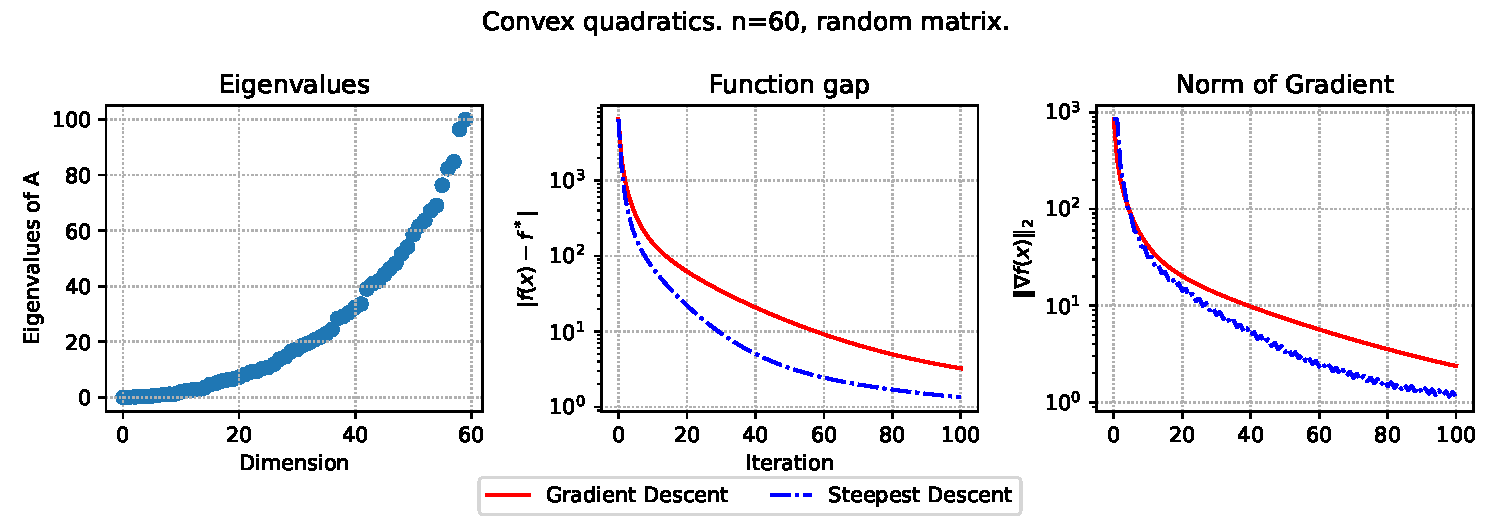
\includegraphics[keepaspectratio]{gd_random_0.001_100_60.pdf}}

\[
f(x) = \frac{1}{2} x^T A x - b^T x \to \min_{x \in \mathbb{R}^n}
\]

\pandocbounded{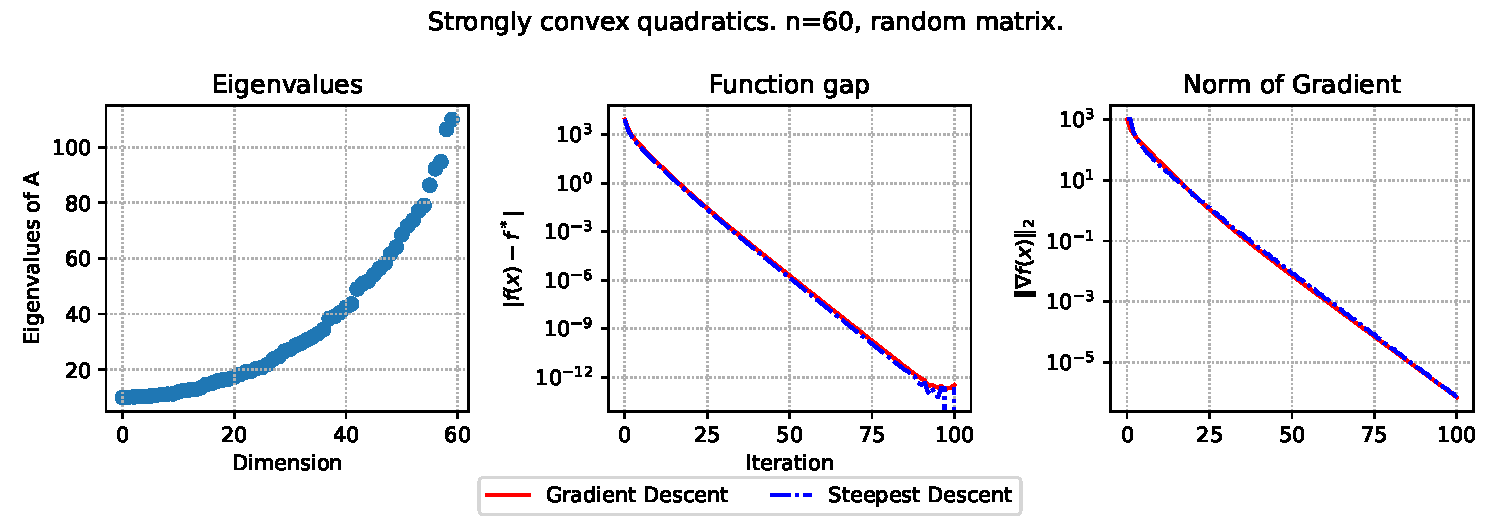
\includegraphics[keepaspectratio]{gd_random_10_100_60.pdf}}

\[
f(x) = \frac{1}{2} x^T A x - b^T x \to \min_{x \in \mathbb{R}^n}
\]

\pandocbounded{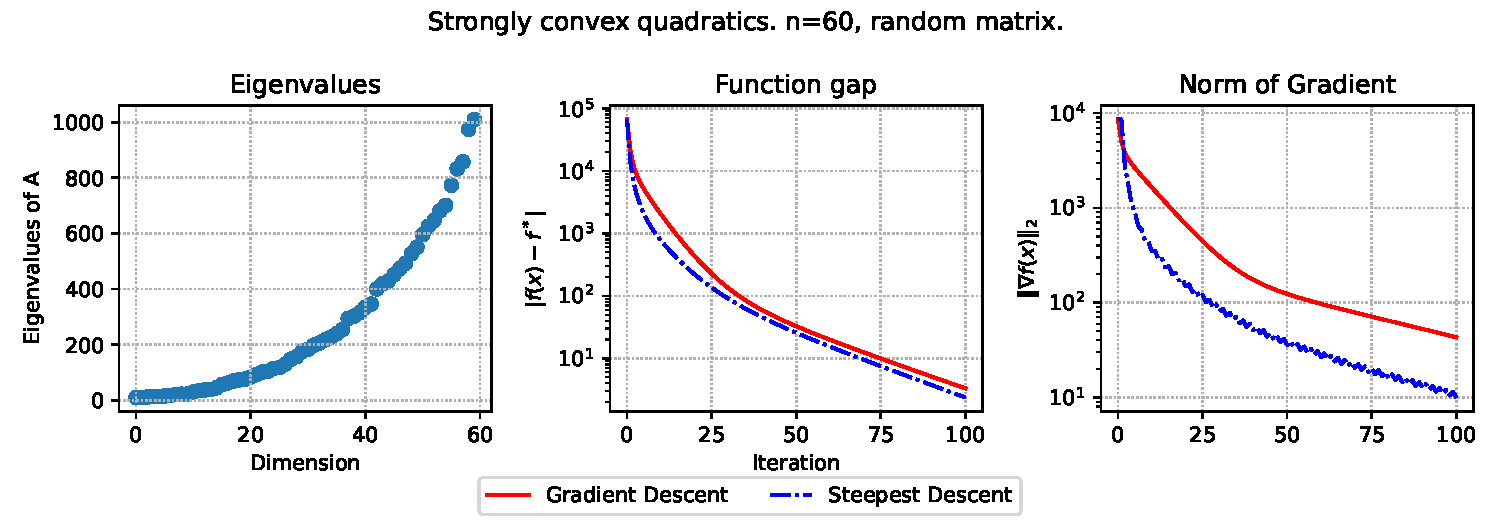
\includegraphics[keepaspectratio]{gd_random_10_1000_60.pdf}}

\[
f(x) = \frac{1}{2} x^T A x - b^T x \to \min_{x \in \mathbb{R}^n}
\]

\pandocbounded{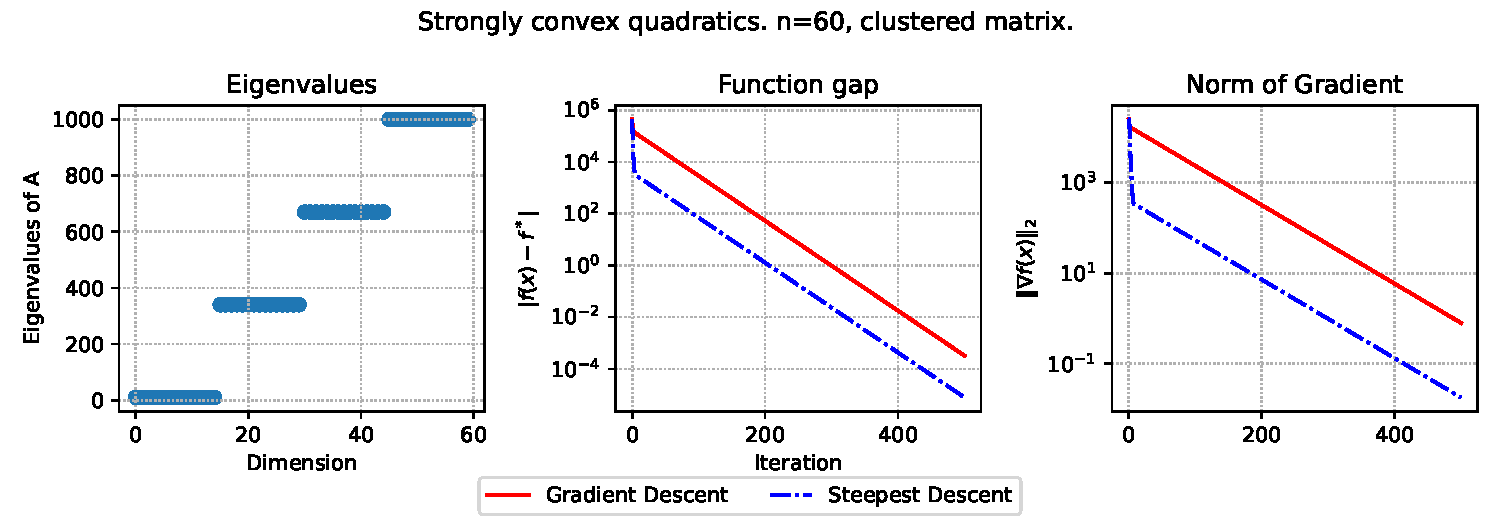
\includegraphics[keepaspectratio]{gd_clustered_10_1000_60.pdf}}

\[
f(x) = \frac{1}{2} x^T A x - b^T x \to \min_{x \in \mathbb{R}^n}
\]

\pandocbounded{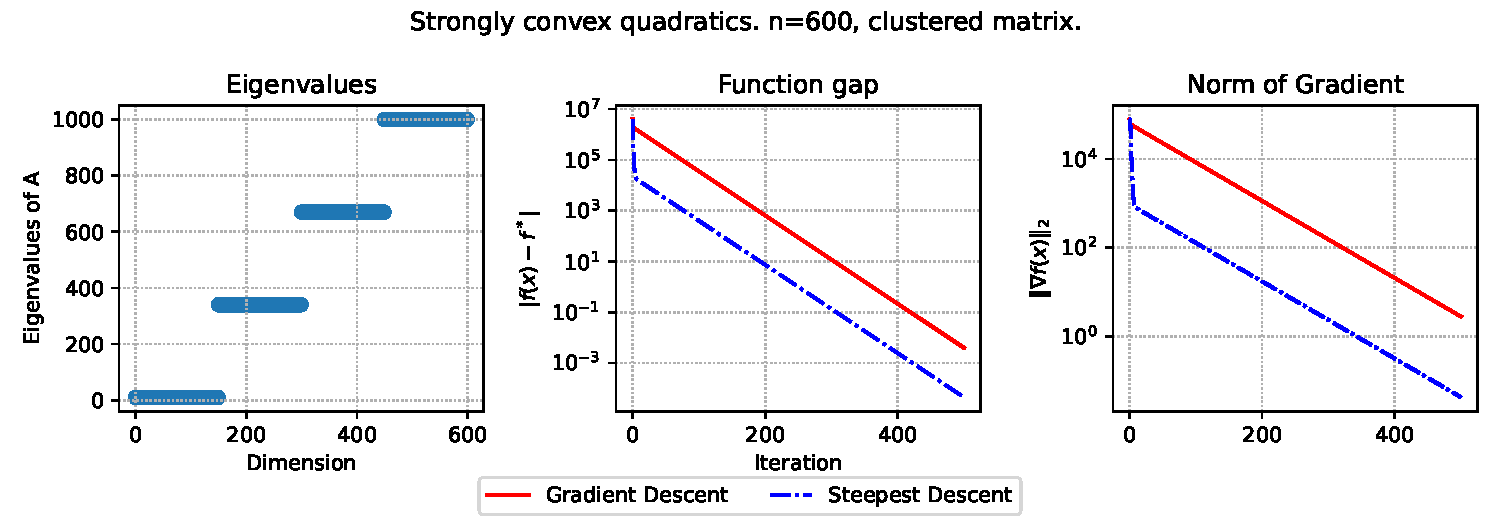
\includegraphics[keepaspectratio]{gd_clustered_10_1000_600.pdf}}

\[
f(x) = \frac{1}{2} x^T A x - b^T x \to \min_{x \in \mathbb{R}^n}
\]

\pandocbounded{\includegraphics[keepaspectratio]{"gd_uniform spectrum_1_100_60.pdf"}}

\[
f(x) = \frac{1}{2} x^T A x - b^T x \to \min_{x \in \mathbb{R}^n}
\]

\pandocbounded{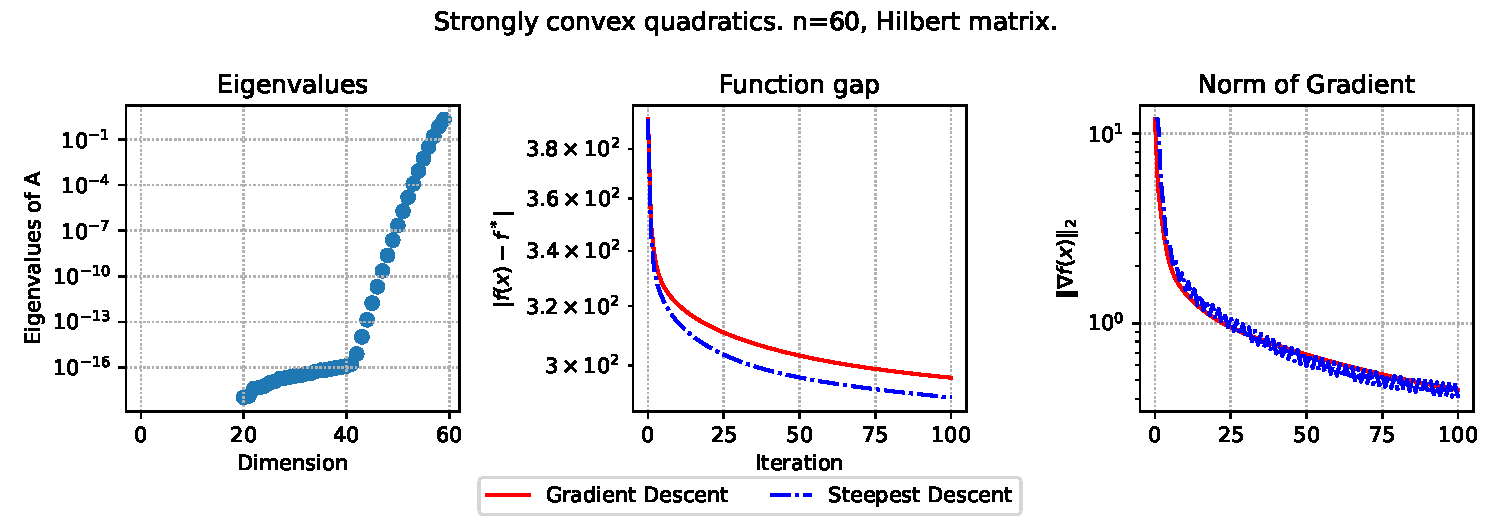
\includegraphics[keepaspectratio]{gd_Hilbert_1_10_60.pdf}}

\[
f(x) = \frac{\mu}{2} \|x\|_2^2 + \frac1m \sum_{i=1}^m \log (1 + \exp(- y_i \langle a_i, x \rangle)) \to \min_{x \in \mathbb{R}^n}
\]

\begin{center}
\includegraphics[width=0.95\linewidth,height=\textheight,keepaspectratio]{"GD 0.07GD 0.9GD 10.0_0.pdf"}
\end{center}

\[
f(x) = \frac{\mu}{2} \|x\|_2^2 + \frac1m \sum_{i=1}^m \log (1 + \exp(- y_i \langle a_i, x \rangle)) \to \min_{x \in \mathbb{R}^n}
\]

\begin{center}
\includegraphics[width=0.95\linewidth,height=\textheight,keepaspectratio]{"GD 0.12GD 0.14GD 0.15_0.1.pdf"}
\end{center}

\[
f(x) = \frac{\mu}{2} \|x\|_2^2 + \frac1m \sum_{i=1}^m \log (1 + \exp(- y_i \langle a_i, x \rangle)) \to \min_{x \in \mathbb{R}^n}
\]

\pandocbounded{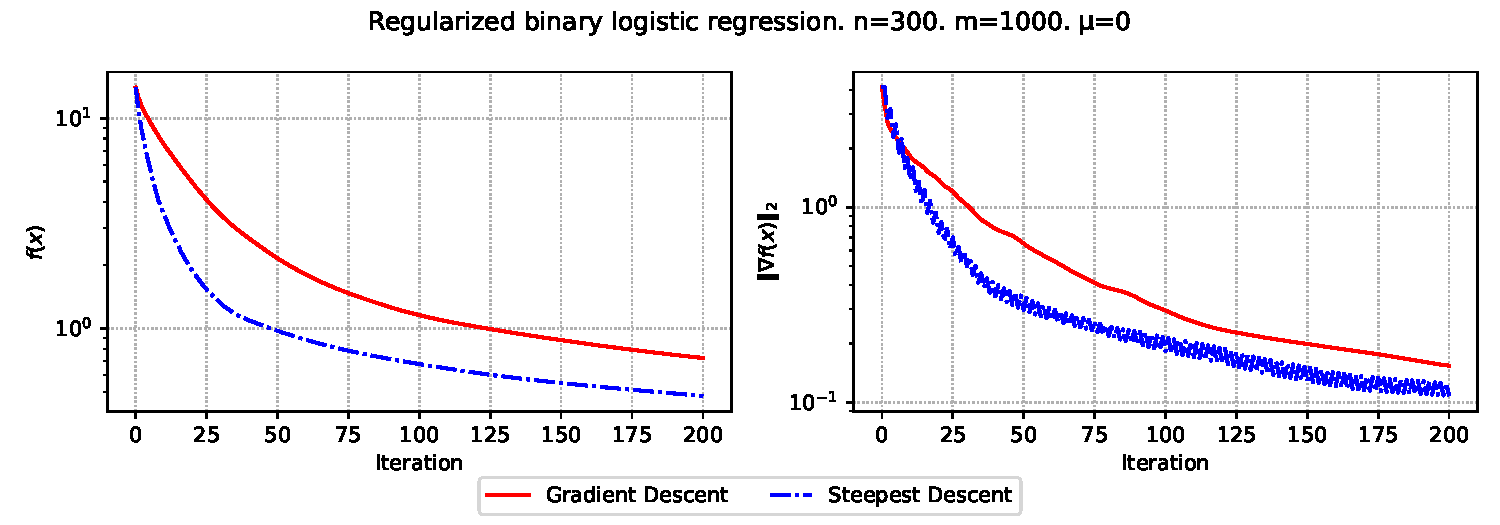
\includegraphics[keepaspectratio]{gd_non_linear_1000_300_0_None.pdf}}

\[
f(x) = \frac{\mu}{2} \|x\|_2^2 + \frac1m \sum_{i=1}^m \log (1 + \exp(- y_i \langle a_i, x \rangle)) \to \min_{x \in \mathbb{R}^n}
\]

\pandocbounded{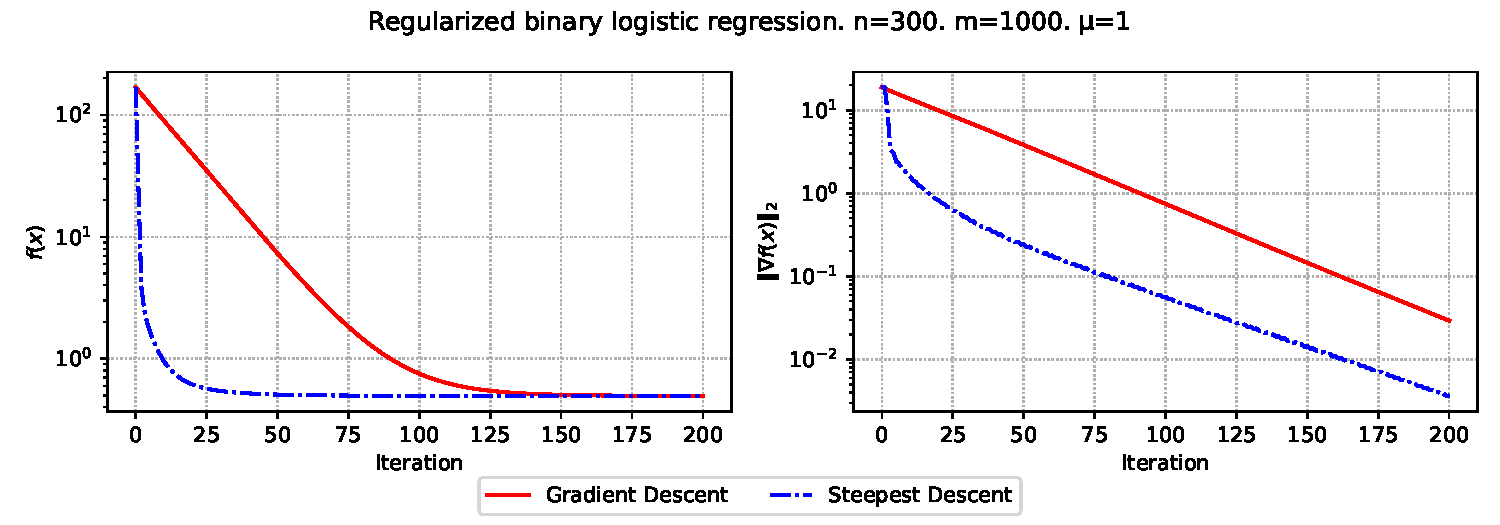
\includegraphics[keepaspectratio]{gd_non_linear_1000_300_1_None.pdf}}

\section{Задачи}\label{ux437ux430ux434ux430ux447ux438}

Рассмотрим задачу \[
    \min_{x \in \mathbb R^n} f(x),
\] где \(f(x)\) выпукла и \(L\)-гладкая. Найдите скорость сходимости
градиентного спуска с оптимальным теоретическим шагом
\(\eta_k = \frac{1}{L}\) для \textit{усредненной точки} и для
\textit{лучшей точки}. Другими словами, получите верхние границы на

\begin{itemize}
\tightlist
\item
  \(f(\bar{x}_N) - f^*,\ \text{where}\ \bar{x}_N = \frac{1}{N} \sum_{i=0}^{N-1} x_i\),
\item
  \(\min_{0 \le i \le N-1} f(x_i) - f^*\).
\end{itemize}

\begin{tcolorbox}[enhanced jigsaw, bottomrule=.15mm, coltitle=black, opacitybacktitle=0.6, colbacktitle=quarto-callout-note-color!10!white, colback=white, opacityback=0, toprule=.15mm, bottomtitle=1mm, toptitle=1mm, arc=.35mm, title=\textcolor{quarto-callout-note-color}{\faInfo}\hspace{0.5em}{Шаг градиентного спуска}, titlerule=0mm, rightrule=.15mm, leftrule=.75mm, left=2mm, colframe=quarto-callout-note-color-frame, breakable]

\[
x_{k + 1} = \arg \min_{x \in \mathbb R^n} \left\{ \Psi_k(x) \equiv f(x_k) + \langle \nabla f(x_k), x - x_k \rangle + \frac{L}{2} \| x - x_k \|_2^2 \right\}
\]

\end{tcolorbox}

\begin{tcolorbox}[enhanced jigsaw, bottomrule=.15mm, coltitle=black, opacitybacktitle=0.6, colbacktitle=quarto-callout-tip-color!10!white, colback=white, opacityback=0, toprule=.15mm, bottomtitle=1mm, toptitle=1mm, arc=.35mm, title=\textcolor{quarto-callout-tip-color}{\faLightbulb}\hspace{0.5em}{Совет}, titlerule=0mm, rightrule=.15mm, leftrule=.75mm, left=2mm, colframe=quarto-callout-tip-color-frame, breakable]

Используйте факт, что \(\Psi_k(x)\) является \(L\)-строго выпуклой из-за
квадратичного регуляризатора.

\end{tcolorbox}

\section{Задачи на
дом}\label{ux437ux430ux434ux430ux447ux438-ux43dux430-ux434ux43eux43c}

\subsection{\texorpdfstring{\textbf{Сходимость градиентного спуска в
невыпуклом гладком случае} {[}10
баллов{]}}{Сходимость градиентного спуска в невыпуклом гладком случае {[}10 баллов{]}}}\label{ux441ux445ux43eux434ux438ux43cux43eux441ux442ux44c-ux433ux440ux430ux434ux438ux435ux43dux442ux43dux43eux433ux43e-ux441ux43fux443ux441ux43aux430-ux432-ux43dux435ux432ux44bux43fux443ux43aux43bux43eux43c-ux433ux43bux430ux434ux43aux43eux43c-ux441ux43bux443ux447ux430ux435-10-ux431ux430ux43bux43bux43eux432}

Мы не будем делать никаких предположений о выпуклости функции \(f\). Мы
покажем, что градиентный спуск достигает \(\varepsilon\)-стационарной
точки \(x\), такой что \(\|\nabla f(x)\|_2 \leq \varepsilon\), за
\(O(1/\varepsilon^2)\) итераций. Важное замечание: вы можете
использовать здесь липшицеву параболическую верхнюю оценку:

\begin{equation}\phantomsection\label{eq-quad_ub}{
f(y) \leq f(x) + \nabla f(x)^T (y-x) + \frac{L}{2} \|y-x\|_2^2, \;\;\;
\text{for all $x,y$}.  
}\end{equation}

\begin{itemize}
\item
  Подставьте \(y = x^{k+1} = x^{k} - \alpha \nabla f(x^k), x = x^k\) в
  (Уравнение~\ref{eq-quad_ub}) чтобы показать, что

  \[
    f(x^{k+1}) \leq f(x^k) - \Big (1-\frac{L\alpha}{2} \Big) \alpha \|\nabla f(x^k)\|_2^2.
    \]
\item
  Используйте \(\alpha \leq 1/L\), и преобразуйте предыдущий результат,
  чтобы получить

  \[
    \|\nabla f(x^k)\|_2^2 \leq \frac{2}{\alpha} \left( f(x^k) - f(x^{k+1}) \right).
    \]
\item
  Просуммируйте предыдущий результат по всем итерациям от
  \(1,\ldots,k+1\) чтобы получить

  \[
    \sum_{i=0}^k \|\nabla f(x^{i})\|_2^2 \leq 
    \frac{2}{\alpha} ( f(x^{0}) - f^*).
    \]
\item
  Дайте нижнюю оценку сумме в предыдущем результате, чтобы получить

  \[
    \min_{i=0,\ldots,k} \|\nabla f(x^{i}) \|_2 
    \leq \sqrt{\frac{2}{\alpha(k+1)} (f(x^{0}) - f^*)}, 
    \] что устанавливает желаемую скорость \(O(1/\varepsilon^2)\) для
  достижения \(\varepsilon\)-стационарности.
\end{itemize}

\subsection{\texorpdfstring{\textbf{Как сходится градиентный спуск в
зависимости от числа обусловленности и размерности.} {[}20
баллов{]}}{Как сходится градиентный спуск в зависимости от числа обусловленности и размерности. {[}20 баллов{]}}}\label{ux43aux430ux43a-ux441ux445ux43eux434ux438ux442ux441ux44f-ux433ux440ux430ux434ux438ux435ux43dux442ux43dux44bux439-ux441ux43fux443ux441ux43a-ux432-ux437ux430ux432ux438ux441ux438ux43cux43eux441ux442ux438-ux43eux442-ux447ux438ux441ux43bux430-ux43eux431ux443ux441ux43bux43eux432ux43bux435ux43dux43dux43eux441ux442ux438-ux438-ux440ux430ux437ux43cux435ux440ux43dux43eux441ux442ux438.-20-ux431ux430ux43bux43bux43eux432}

Исследуйте, как количество итераций, необходимое для сходимости
градиентного спуска, зависит от следующих двух параметров: числа
обусловленности \(\kappa \geq 1\) функции, которую мы оптимизируем, и
размерности \(n\) пространства переменных, по которым мы оптимизируем.

Для этого при заданных параметрах \(n\) и \(\kappa\) случайно
сгенерируйте квадратичную задачу размера \(n\) с числом обусловленности
\(\kappa\) и запустите на ней градиентный спуск с заранее заданной
фиксированной точностью. Измерьте число итераций \(T(n,\kappa)\),
которое потребовалось методу для сходимости (успешного завершения по
критерию останова).

Рекомендация: самый простой способ сгенерировать случайную квадратичную
задачу размера \(n\) с заданным числом обусловленности \(\kappa\)
следующий - удобно взять диагональную матрицу \(A \in S_{n}^{++}\) в
виде \(A = \text{Diag}(a)\), где диагональные элементы случайно
выбираются из интервала \([1, \kappa]\) и удовлетворяют \(\min(a) = 1\),
\(\max(a) = \kappa\). В качестве вектора \(b \in \mathbb{R}^n\) можно
взять вектор со случайными компонентами. Диагональные матрицы удобны для
рассмотрения, поскольку их можно эффективно обрабатывать даже при
больших значениях \(n\).

Зафиксируйте определенное значение размерности \(n\). Итерируйте по
различным числам обусловленности \(\kappa\) на сетке и постройте
зависимость \(T(n,\kappa)\) от \(\kappa\). Поскольку квадратичная задача
каждый раз генерируется случайно, повторите этот эксперимент несколько
раз. В результате для фиксированного значения \(n\) вы должны получить
семейство кривых, показывающих зависимость \(T(n, \kappa)\) от
\(\kappa\). Изобразите все эти кривые в одном цвете для ясности
(например, красный).

Увеличьте значение \(n\) и повторите эксперимент. Вы должны получить
новое семейство кривых \(T(n',\kappa)\) от \(\kappa\). Изобразите все
эти кривые в одном цвете, но отличающемся от предыдущего (например,
синий).

Повторите эту процедуру несколько раз для других значений \(n\). В итоге
вы должны получить несколько разных семейств кривых - некоторые красные
(соответствующие одному значению \(n\)), некоторые синие
(соответствующие другому значению \(n\)), некоторые зеленые и т.д.

Обратите внимание, что имеет смысл перебирать значения размерности \(n\)
по логарифмической сетке (например, \(n = 10\), \(n = 100\),
\(n = 1000\) и т. д.). Используйте следующий критерий остановки:
\(\|\nabla f(x_k)\|_2^2 \leq \varepsilon \|\nabla f(x_0)\|_2^2\) при
\(\varepsilon = 10^{-5}\). В качестве начальной точки возьмите
\(x_0 = (1, \ldots, 1)^T\).

Какие выводы можно сделать из полученного рисунка?




\end{document}
